Una empresa de distribución (LogiMax S.A.) quiere conectar sus centros de distribución en distintas ciudades minimizando el coste total de infraestructura de fibra óptica. Cada conexión entre ciudades tiene un coste asociado (en miles de \euro). La empresa quiere construir una red que conecte todos los centros minimizando el coste total. Aplicando y explicando los métodos estudiados en la asignatura, ¿qué red debe construir y qué coste tiene?

% En el preámbulo:
% \usepackage{tikz}

\tikzset{
logiNode/.style={circle, draw=blue!50!black, fill=blue!20, minimum size=0.75cm, font=\small\bfseries},
logiNodeSol/.style={circle, draw=black, very thick, fill=blue!20, minimum size=0.75cm, font=\small\bfseries},
logiEdge/.style={-, thick, draw=gray!70!black},
logiSol/.style={-, line width=2.2pt, draw=black},
logiLabel/.style={sloped, midway, auto, font=\scriptsize, fill=white, inner sep=1pt}
}

\newcommand{\coordLogiMax}{
\coordinate (A) at (7,0.5);
\coordinate (B) at (6.5,3.5);
\coordinate (C) at (3.5,3);
\coordinate (D) at (4.5,5.5);
\coordinate (E) at (1,5);
\coordinate (F) at (2.7,8);
\coordinate (G) at (1,1.5);
\coordinate (H) at (8.5,5.5);
\coordinate (I) at (-0.5,-0.5);
}

\newcommand{\aristasLogiMax}{
\draw[logiEdge] (A)--(B);
\draw[logiEdge] (A)--(C);
\draw[logiEdge] (B)--(D);
\draw[logiEdge] (B)--(C);
\draw[logiEdge] (B)--(H);
\draw[logiEdge] (C)--(E);
\draw[logiEdge] (C)--(G);
\draw[logiEdge] (D)--(F);
\draw[logiEdge] (D)--(E);
\draw[logiEdge] (D)--(C);
\draw[logiEdge] (E)--(F);
\draw[logiEdge] (E)--(G);
\draw[logiEdge] (F)--(H);
\draw[logiEdge] (G)--(I);
}

\newcommand{\pesosLogiMax}{
\path (A)--node[logiLabel]{4}(B);
\path (A)--node[logiLabel]{3}(C);
\path (B)--node[logiLabel]{2}(D);
\path (B)--node[logiLabel]{1}(C);
\path (B)--node[logiLabel]{5}(H);
\path (C)--node[logiLabel]{5}(E);
\path (C)--node[logiLabel]{1}(G);
\path (D)--node[logiLabel]{6}(F);
\path (D)--node[logiLabel]{1}(E);
\path (D)--node[logiLabel]{4}(C);
\path (E)--node[logiLabel]{2}(F);
\path (E)--node[logiLabel]{3}(G);
\path (F)--node[logiLabel]{4}(H);
\path (G)--node[logiLabel]{4}(I);
}

\newcommand{\nodosLogiMax}{
\foreach \n in {A,B,C,D,E,F,G,H,I}{
\node[logiNode] at (\n) {$\n$};
}
}

\newcommand{\grafoLogiMaxBase}{
\begin{center}
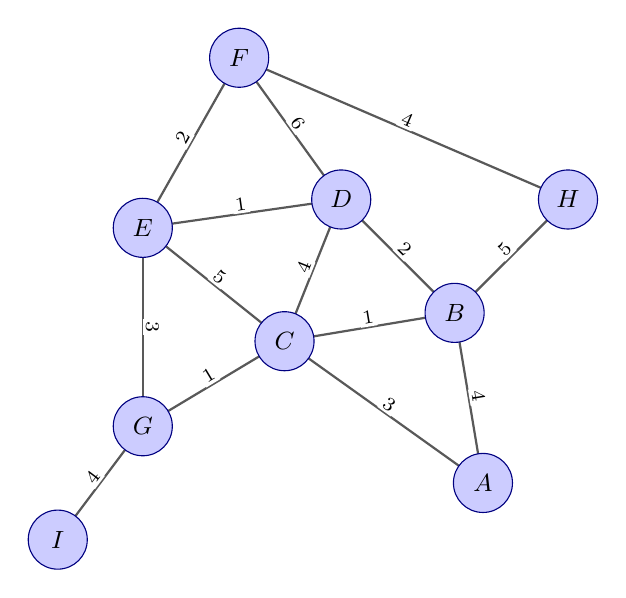
\begin{tikzpicture}[scale=0.72]
\coordLogiMax
\aristasLogiMax
\pesosLogiMax
\nodosLogiMax
\end{tikzpicture}
\end{center}
}

\newcommand{\grafoLogiMaxSeleccion}[2]{
\begin{center}
\begin{tikzpicture}[scale=0.72]
\coordLogiMax
\aristasLogiMax
#1
\pesosLogiMax
\nodosLogiMax
\foreach \n in {#2}{
\node[logiNodeSol] at (\n) {$\mathbf{\n}$};
}
\end{tikzpicture}
\end{center}
}

\textbf{Solución}

El problema consiste en conectar todos los centros de distribución con coste mínimo. Por tanto, se trata de un problema de árbol generador mínimo. Para resolverlo se aplica el algoritmo de Kruskal (alternativamente, se puede usar el algoritmo de Prin).

El algoritmo de Kruskal consiste en ordenar las aristas de menor a mayor coste e ir incorporándolas a la solución siempre que no formen un ciclo. El procedimiento termina cuando se han seleccionado $n-1$ aristas, donde $n$ es el número de vértices. En este caso hay $9$ vértices, por lo que el árbol generador mínimo debe tener $8$ aristas.

\begin{enumerate}
\item \textbf{Paso 1. Ordenación de las aristas.}


Se ordenan las conexiones de menor a mayor coste. Un posible orden compatible con los costes es el siguiente:

\[
\begin{array}{c|c|c}
\text{Orden} & \text{Arista} & \text{Coste}\\
\hline
1 & BC & 1\\
2 & CG & 1\\
3 & DE & 1\\
4 & BD & 2\\
5 & EF & 2\\
6 & AC & 3\\
7 & EG & 3\\
8 & AB & 4\\
9 & CD & 4\\
10 & FH & 4\\
11 & GI & 4\\
12 & BH & 5\\
13 & CE & 5\\
14 & DF & 6
\end{array}
\]

En caso de empate entre aristas con el mismo coste, se puede escoger cualquiera de ellas, siempre que no se forme ciclo.

\grafoLogiMaxBase

\item \textbf{Paso 2. Selección de la arista $BC$.}

La arista de menor coste es $BC$, con coste $1$. Se incorpora a la solución porque conecta dos vértices que todavía no estaban unidos.

\[
T=\{BC\}.
\]

\grafoLogiMaxSeleccion{
    \draw[logiSol] (B)--(C);
}{B,C}

\item \textbf{Paso 3. Selección de la arista $CG$.}

La siguiente arista de menor coste es $CG$, con coste $1$. Se incorpora porque no forma ciclo con las aristas ya seleccionadas.

\[
T=\{BC,CG\}.
\]

\grafoLogiMaxSeleccion{
    \draw[logiSol] (B)--(C);
    \draw[logiSol] (C)--(G);
}{B,C,G}

\item \textbf{Paso 4. Selección de la arista $DE$.}

La siguiente arista de coste mínimo es $DE$, con coste $1$. Se incorpora porque conecta dos vértices que forman una nueva componente y no genera ningún ciclo.

\[
T=\{BC,CG,DE\}.
\]

\grafoLogiMaxSeleccion{
    \draw[logiSol] (B)--(C);
    \draw[logiSol] (C)--(G);
    \draw[logiSol] (D)--(E);
}{B,C,D,E,G}

\item \textbf{Paso 5. Selección de la arista $BD$.}

La arista $BD$ tiene coste $2$. Se incorpora porque une la componente formada por $B,C,G$ con la componente formada por $D,E$.

\[
T=\{BC,CG,DE,BD\}.
\]

\grafoLogiMaxSeleccion{
    \draw[logiSol] (B)--(C);
    \draw[logiSol] (C)--(G);
    \draw[logiSol] (D)--(E);
    \draw[logiSol] (B)--(D);
}{B,C,D,E,G}

\item \textbf{Paso 6. Selección de la arista $EF$.}

La arista $EF$ tiene coste $2$. Se incorpora porque conecta el vértice $F$ con la componente ya construida y no forma ciclo.

\[
T=\{BC,CG,DE,BD,EF\}.
\]

\grafoLogiMaxSeleccion{
    \draw[logiSol] (B)--(C);
    \draw[logiSol] (C)--(G);
    \draw[logiSol] (D)--(E);
    \draw[logiSol] (B)--(D);
    \draw[logiSol] (E)--(F);
}{B,C,D,E,F,G}

\item \textbf{Paso 7. Selección de la arista $AC$.}

La arista $AC$ tiene coste $3$. Se incorpora porque conecta el vértice $A$ con la componente ya construida.

\[
T=\{BC,CG,DE,BD,EF,AC\}.
\]

\grafoLogiMaxSeleccion{
    \draw[logiSol] (B)--(C);
    \draw[logiSol] (C)--(G);
    \draw[logiSol] (D)--(E);
    \draw[logiSol] (B)--(D);
    \draw[logiSol] (E)--(F);
    \draw[logiSol] (A)--(C);
}{A,B,C,D,E,F,G}

\item \textbf{Paso 8. Descarte de aristas que forman ciclo y selección de $FH$.}

La arista $EG$, de coste $3$, no se incorpora porque sus extremos ya están conectados en la solución parcial y formaría un ciclo. También se descartan $AB$ y $CD$, de coste $4$, por el mismo motivo.

La arista $FH$, de coste $4$, sí se incorpora porque conecta el vértice $H$ con la componente ya construida.

\[
T=\{BC,CG,DE,BD,EF,AC,FH\}.
\]

\grafoLogiMaxSeleccion{
    \draw[logiSol] (B)--(C);
    \draw[logiSol] (C)--(G);
    \draw[logiSol] (D)--(E);
    \draw[logiSol] (B)--(D);
    \draw[logiSol] (E)--(F);
    \draw[logiSol] (A)--(C);
    \draw[logiSol] (F)--(H);
}{A,B,C,D,E,F,G,H}

\item \textbf{Paso 9. Selección de la arista $GI$.}

La arista $GI$ tiene coste $4$. Se incorpora porque conecta el último vértice que falta, $I$, con la red ya construida.

\[
T=\{BC,CG,DE,BD,EF,AC,FH,GI\}.
\]

\grafoLogiMaxSeleccion{
    \draw[logiSol] (B)--(C);
    \draw[logiSol] (C)--(G);
    \draw[logiSol] (D)--(E);
    \draw[logiSol] (B)--(D);
    \draw[logiSol] (E)--(F);
    \draw[logiSol] (A)--(C);
    \draw[logiSol] (F)--(H);
    \draw[logiSol] (G)--(I);
}{A,B,C,D,E,F,G,H,I}

\item \textbf{Paso 10. Comprobación de finalización.}

Ya se han seleccionado $8$ aristas, que es el número necesario para conectar $9$ vértices sin formar ciclos. Por tanto, el algoritmo termina.

La red que debe construir LogiMax S.A. está formada por las siguientes conexiones:

\[
\boxed{
T=\{BC,CG,DE,BD,EF,AC,FH,GI\}.
}
\]

El coste total es:

\[
1+1+1+2+2+3+4+4=18.
\]

Por tanto, el coste mínimo de infraestructura es:

\[
\boxed{18\text{ miles de euros}}.
\]

% Equivalentemente, el coste total es:

% \[
% \boxed{18000\text{ euros}}.
% \]

\end{enumerate}
